%====================================================
%
% Author: Dipl.--Inf. XAVIER NOUMBISSI NOUNDOU
%
%====================================================
\documentclass[a4paper, 10pt]{article}
\NeedsTeXFormat{LaTeX2e}

%---------------------------- PACKAGE INCLUSION -------------------------------
% This group renders characters clearer and more precise

\RequirePackage[bitstream-charter,cal,expert]{mathdesign}
\RequirePackage{latexsym}

\usepackage[numbib]{tocbibind}

\usepackage{geometry}
\geometry{a4paper,
		  %showframe=true,
		  %margin=2.75em,
		  %a4paper,
		  %total={170mm,257mm},
		  top=4.3em,
		  left=3em,
		  right=3em,
		  bottom=3.39em
		  }

\usepackage{graphicx}  

\usepackage{multicol}  	  

\usepackage{caption}

\usepackage[default]{cantarell}
\usepackage{graphicx}
\usepackage{xspace}
\usepackage[parfill]{parskip} % Activate to begin paragraphs with an empty line rather than an indent
\usepackage{paralist} % very flexible & customisable lists (eg. enumerate/itemize, etc.)
\usepackage{listings} % for lstset definitions
\usepackage{url}
\usepackage{subfig} % make it possible to include more than one captioned figure/table in a single float
\usepackage{epsfig}
\usepackage{booktabs}
%\usepackage{enumitem} %funny itemize icons
\usepackage{verbatim}
\usepackage{tcolorbox}

\usepackage{pagecolor}

\usepackage{amsmath}
\newcommand{\mathbold}[1]{\text{\textbf{#1}}}

\usepackage{xcolor}
\definecolor{yerothColorOrange}{RGB}{242, 161, 0}   
\definecolor{yerothColorBlue}{RGB}{77 , 93 , 254}
\definecolor{yerothColorRed}{RGB}{254, 48 , 48}
\definecolor{yerothColorGray}{RGB}{198, 198, 198}
\definecolor{yerothColorDarkgray}{RGB}{60, 60 , 60}
\definecolor{yerothColorIndigo}{RGB}{83, 0, 125}
\definecolor{yerothColorGreen}{RGB}{2  , 160, 70}
\definecolor{forestgreen}{RGB}{2,160,70}    
\definecolor{mediumblue}{RGB}{7,43,205}    
\definecolor{firebrickred}{RGB}{178,34,34}
\definecolor{listingray}{gray}{0.9}
\definecolor{lbcolor}{rgb}{0.9,0.9,0.9}
\definecolor{darkgreen}{rgb}{0,0.35,0}
\definecolor{medgreen}{rgb}{0,0.5,0}
\definecolor{lightgreen}{rgb}{0.5,0.7,0.5}
\definecolor{pmcolour}{rgb}{0.5,0.7,0.5}
\definecolor{medgrey}{rgb}{0.6,0.6,0.6}
\definecolor{purplish}{rgb}{0.4,0,0.6}
\definecolor{brightred}{rgb}{1,0.2,0.2}

\newcommand{\diplinfn}{Dipl.--Inf.\xspace}

\newcommand{\yerothrd}{\textcolor{yerothColorGreen}
			{\textsc{\textcolor{yerothColorRed}{YEROTH}}$_{\text{r\&d}}$\xspace}}

\newcommand{\mytime}[2]{$#1$:$#2$\xspace}

\newcommand{\webbrowserbased}{web--browser--based\xspace}

\newcommand{\yerotherpblack}{YEROTH--ERP--$3.0$\xspace}

\newcommand{\yerotherp}{\textsc{\textcolor{yerothColorBlue}{YEROTH--ERP--$3.0$}}\xspace}

\newcommand{\saperp}{'SAP Business One'\xspace}

\newcommand{\sageerp}{'Sage Gescom i$7$'\xspace}

\newcommand{\myfullacademicname}{Dipl.--Inf. XAVIER NOUMBISSI NOUNDOU\xspace}

\usepackage{hyperref}
\hypersetup{
    colorlinks,
	pagebackref,
    citecolor=medgreen,
    linkcolor=purplish,
    breaklinks,
    pdftex,
    bookmarks,
    plainpages=false,
	pdftitle={The application architecture of \yerotherpblack.
			Authored by: ''\myfullacademicname''.},
    pdfauthor={\myfullacademicname}
}

%--------------------------------------------------------------------------------

%---------------------------- COMMANDS DEFINITION -------------------------------
\newcommand{\diplinf}{\emph{Dipl.-Inf.}\xspace}
\newcommand{\mycheckmark}[1]{\textcolor{#1}{$\checkmark$}\xspace}

\newcommand{\myenumitem}[1]{\emph{#1}\xspace}
\newcommand{\yerenalert}{\emph{yeren-alert}\xspace}

\newcommand{\erpsoftware}{ERP~software--system\xspace}

\newcommand{\wy}{WYSIWYG\xspace}

\newcommand{\applicationtier}[1]{$#1$--tier\xspace}

\newcommand{\thickclient}{thick--client\xspace}

\newcommand{\ministudio}{\texttt{miniStudio (vxWorks)}\xspace}

\newcommand{\qtdesigner}{\texttt{Qt designer}\xspace}

\newcommand{\cplusplus}{\texttt{C++}\xspace}


\newcommand{\yerothvert}[1]{\textcolor{yerothColorGreen}{#1}\xspace}
\newcommand{\yerothrouge}[1]{\textcolor{yerothColorRed}{#1}\xspace}

\newcommand{\featuresummary}[2]{\textbf{\textcolor{#1}{\textsc{#2}}}}

%--------------------------------------------------------------------------------

\usepackage[T1]{fontenc}
\newcommand{\changefont}[3]{
\fontfamily{#1} \fontseries{#2} \fontshape{#3} \selectfont}
\changefont{cmss}{m}{n}

\renewcommand\labelenumi{\theenumi)}

\pagenumbering{arabic}

\usepackage{fancyhdr}
\pagestyle{fancy}
\renewcommand{\headrulewidth}{0pt}
\rhead{\textbf{\yerothrd}}
\lhead{The Application Architecture of \yerotherpblack}
\lfoot{{\small Author: \myfullacademicname}}
\rfoot{{\small Version of --~\today~--}}
\cfoot{\thepage}

\clubpenalty = 10000
\widowpenalty = 10000
\displaywidowpenalty = 10000

\fancypagestyle{OnlyFirstPage}{%
	\lhead{}
	\rhead{}
    \lfoot{}
}

\begin{document}

\thispagestyle{OnlyFirstPage}

{\bf \Large \yerothrd} {| \sc \scriptsize the application architecture of \yerotherpblack}

\vspace{2.0em}

\begin{center}
{\LARGE The Application Architecture of \yerotherpblack}
\end{center}

\vspace{2.0em}

\begin{center}
{\large \myfullacademicname}
\end{center}

\vspace{2.0em}

\begin{abstract}
\begin{center}
\parbox{42em}{
This document describes the architecture of our
\erpsoftware \yerotherpblack.
This document also explains the reasons for our
choice to design and build \yerotherpblack as
a \thickclient application, as opposed to
currently more popular \webbrowserbased
applications.
}
\end{center}
\end{abstract}

\vspace{5em}

% TABLE OF CONTENTS
\phantomsection
\addcontentsline{toc}{section}{\contentsname}
\begingroup
\tableofcontents
\endgroup

\newpage

\begin{multicols}{2}

\end{multicols}

\begin{table*}[!htbp]
\centering
\resizebox{\textwidth}{!}{%to fit the table within the text width
\begin{tabular}{cccc} 

\multicolumn{1}{c}{}			&
Thick--client application 		& 
Web--browser--based application	\\ \hline

application business code installation and upgrade	&
		\yerothrouge{on each computer}				&						
		\yerothvert{only on the web~/~application server}	\\ \hline
		
user interface installation and upgrade				&
		\yerothvert{on each computer}				&						
		\yerothvert{on each computer}				\\ \hline		

user interface development			&
		\yerothvert{WYSIWYG tool}	&						
		\yerothrouge{manual coding}	\\ \hline

application networked architecture				&
		\yerothvert{1--tier architecture}		&						
		\yerothrouge{multi--tier architecture}	\\ \hline

other involved software--systems				&
		\yerothvert{at least $1$ (DBMS)}		&						
		\yerothrouge{at least $2$ (DBMS, web~/~application server)}	\\
\end{tabular}}
\caption{Thick--client application VS Web--browser--based application\\}
\label{tab:thickclient-application-againts-webbrowserbased-application}
\end{table*}

\begin{multicols}{2}


\section{Introduction}
\yerotherpblack is an \textbf{Enterprise Resource Planing (ERP)}
software that aims 'effectiveness' and 'simplicity',
compared to other high ranked ERP software--systems
(e.g.: \sageerp, \saperp, etc.).

We chose to design and implement \yerotherpblack as
a \thickclient software--system because of the
following reasons:

\begin{enumerate}
	\item the implementation language \cplusplus
		offers much flexibility (use of macro, etc.)
		
	\item the availability of \texttt{'WHAT YOU SEE IS WHAT YOU GET'}
		(\wy) tools for fast and useful
		user interface design (e.g.: \qtdesigner~\cite{qtdesigner:2020},
		\ministudio~\cite{miniStudio:2020}, etc.)
		
	\item the low number of computers involved
		with the operation of a \thickclient
		software--system (\applicationtier{1} architecture),
		as opposed to a \webbrowserbased software--system
		(at least a \applicationtier{2} architecture).
	
\end{enumerate}

%%%%%%%%%%%%%%%%%%%%%%%%%%%%%%%%%%%%%%%%%%%%%%%%%%%%%%%%%%%%%%%%%%%%%%%%%%%


\section{Thick--Client VS Web--Browser}

\begin{center}
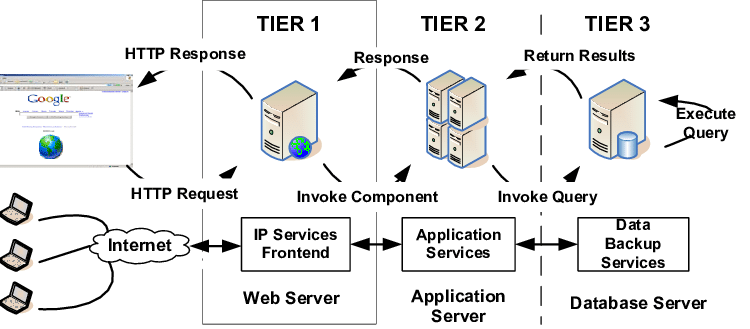
\includegraphics[scale=0.39]{images/yeroth-three-tier-architecture.png}
\captionof{figure}{Physical \applicationtier{3} architecture.}
\label{fig:yeroth-three-tier-architecture}
\end{center}

Figure~\ref{fig:yeroth-three-tier-architecture}
illustrates an example of a physical
\applicationtier{3} architecture
(copied from \cite{trevor:2006}).

\vspace{1em}

\begin{center}
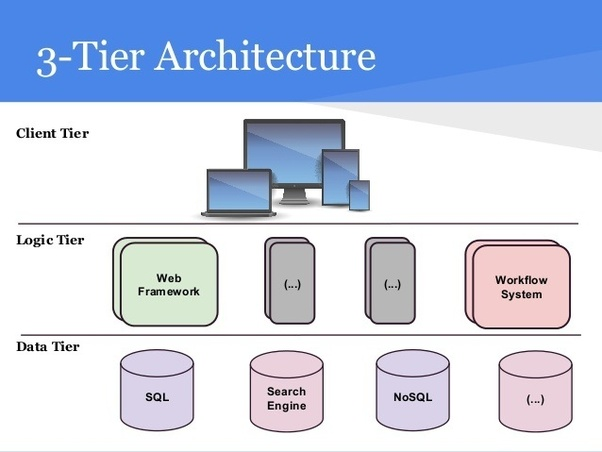
\includegraphics[scale=0.42]{images/yeroth-three-tier-architecture-logical.png}
\captionof{figure}{Logical \applicationtier{3} architecture.}
\label{fig:yeroth-three-tier-architecture-logical}
\end{center}

Figure~\ref{fig:yeroth-three-tier-architecture-logical}
illustrates an example of a logical
\applicationtier{3} architecture 
(copied from \cite{quoradotcom:2020}).

\vspace{1em}

Table~\ref{tab:thickclient-application-againts-webbrowserbased-application}
compares a \thickclient application against
a \webbrowserbased application.




%%%%%%%%%%%%%%%%%%%%%%%%%%%%%%%%%%%%%%%%%%%%%%%%%%%%%%%%%%%%%%%%%%%%%%%%%%%


\section{\yerotherpblack Upgrade Deployment}


\subsection{Debian--Linux}


\subsection{Windows~$10$}



\section{Conclusion}


\newpage


\bibliographystyle{alpha}
\bibliography{yeroth-erp-3-0-application-architecture}

\end{multicols}

\end{document}

